En el proceso de elaboración se incluyen las tareas relacionadas con la arquitectura del sistema, y se genera una base ejecutable del código sobre la cual se pueda 
empezar a testear dicha arquitectura.

Al mismo tiempo se desarrollan los componentes con un rol central dentro de la arquitectura definida, y los módulos de los casos de uso con más riesgos
de alto impacto a nivel estructural, dejando cada una en una iteración diferente. La idea es construir la arquitectura de forma incremental. La opción a nivel arquitectura propuesta
en cada iteración debe ser compatible con la anterior, y al mismo tiempo solucionar el caso de uso actual.

\begin{figure}[h!]
   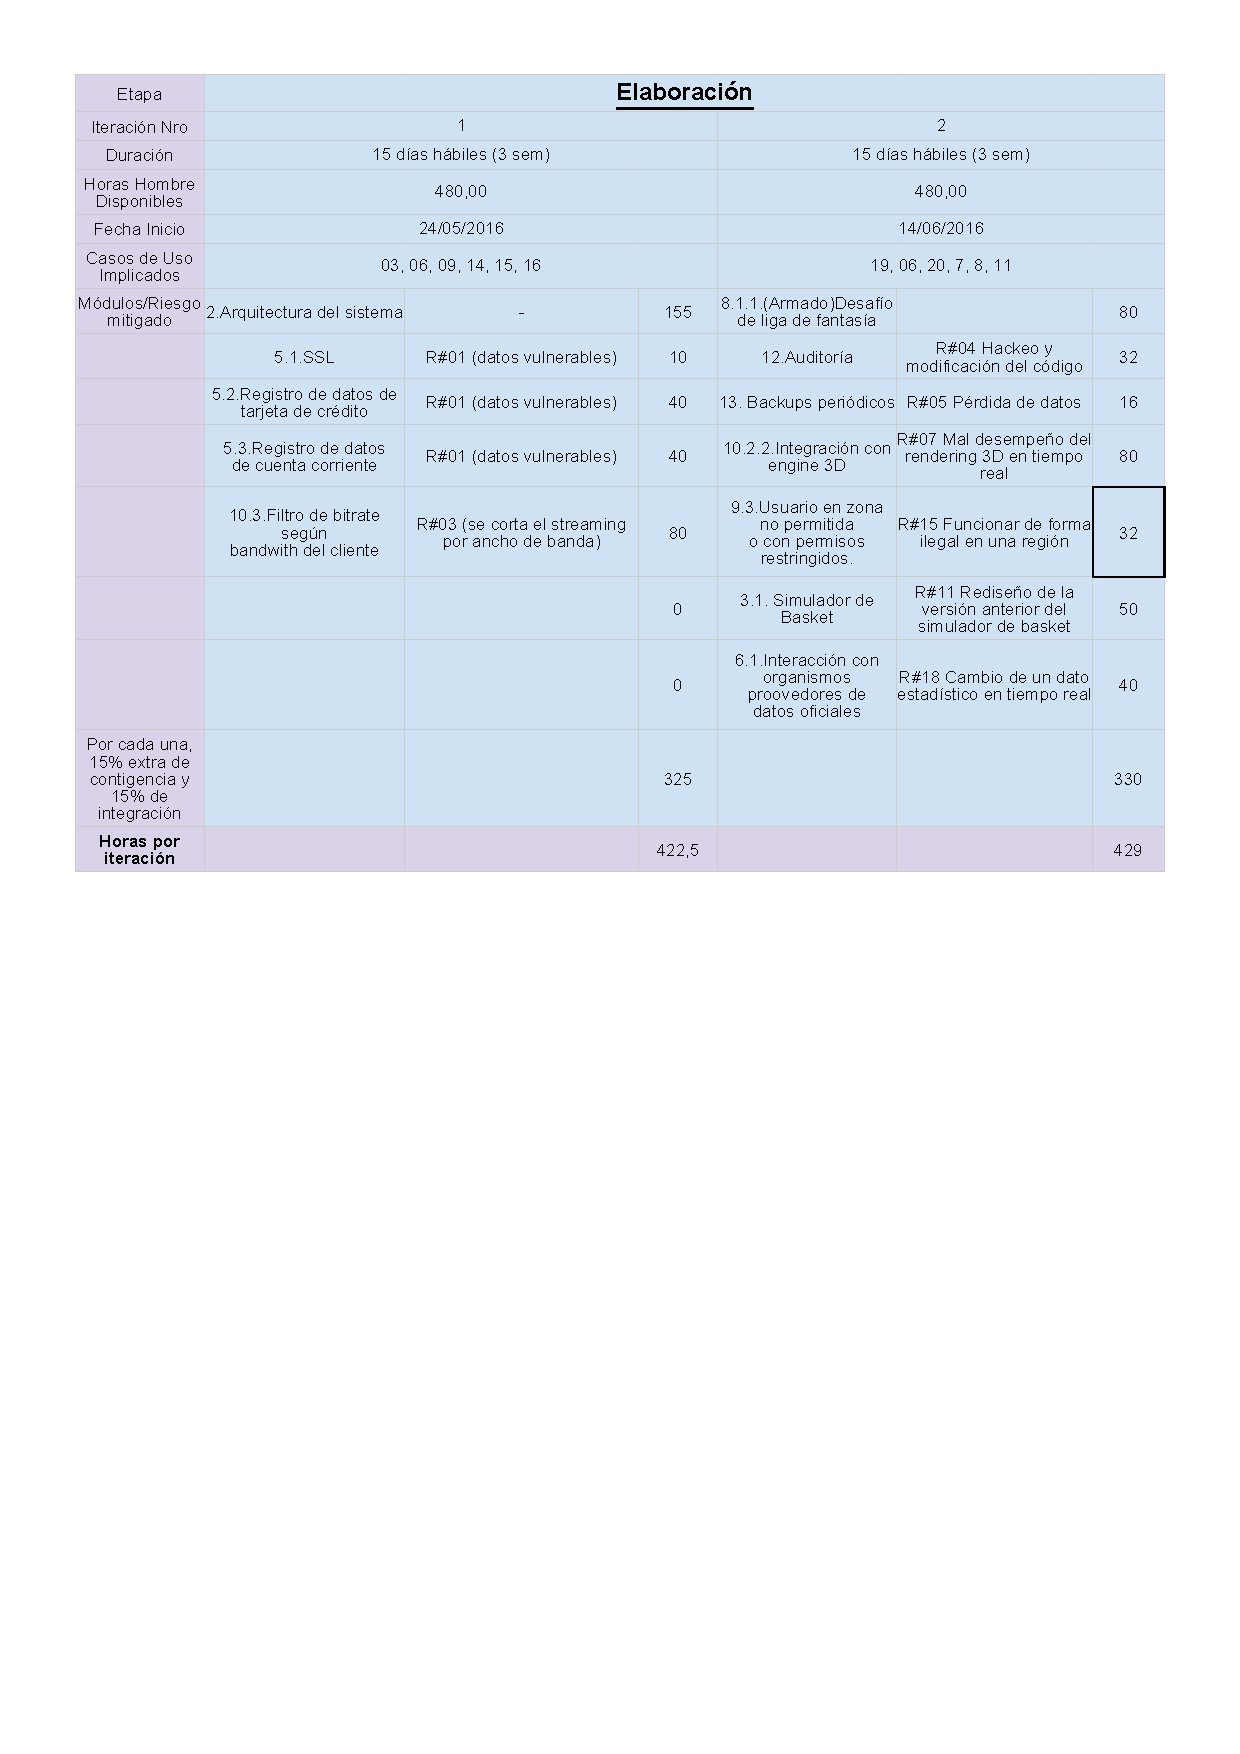
\includegraphics[scale=0.80]{imagenes/etapas-elaboracion.pdf}
   \caption{División de tareas en la etapa de elaboración}
\end{figure}

En la etapa de construcción se desarrollan los módulos y casos de uso faltantes faltantes de forma iterativa incremental. 

Finalmente en la etapa de transición se realizan tareas de mantenimiento.

\newpage
\begin{landscape}

\begin{figure}[h!]
   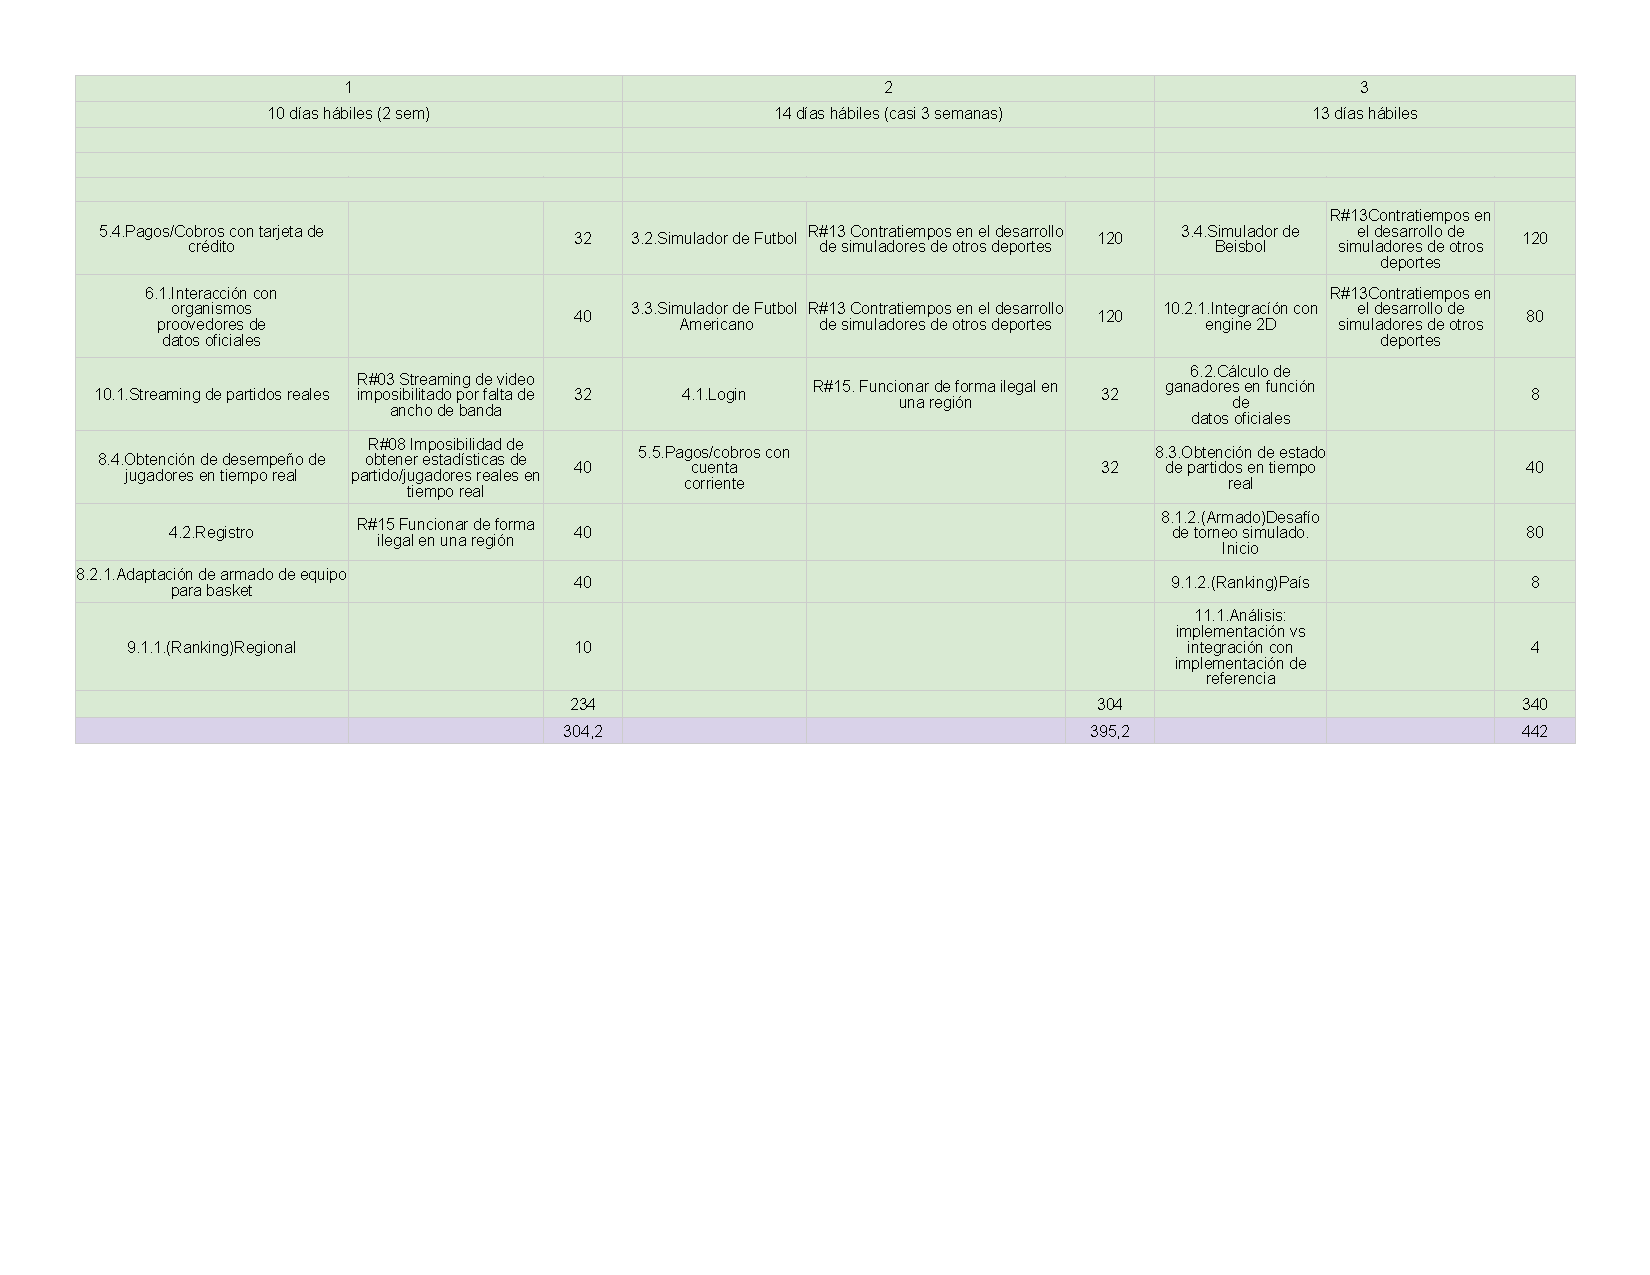
\includegraphics[scale=0.8]{imagenes/construccion123.pdf}
   \caption{División de tareas de las primeras 3 iteraciones de la etapa de 'Construcción'}
\end{figure}

\end{landscape}
\newpage

\newpage
\begin{landscape}

\begin{figure}[h!]
   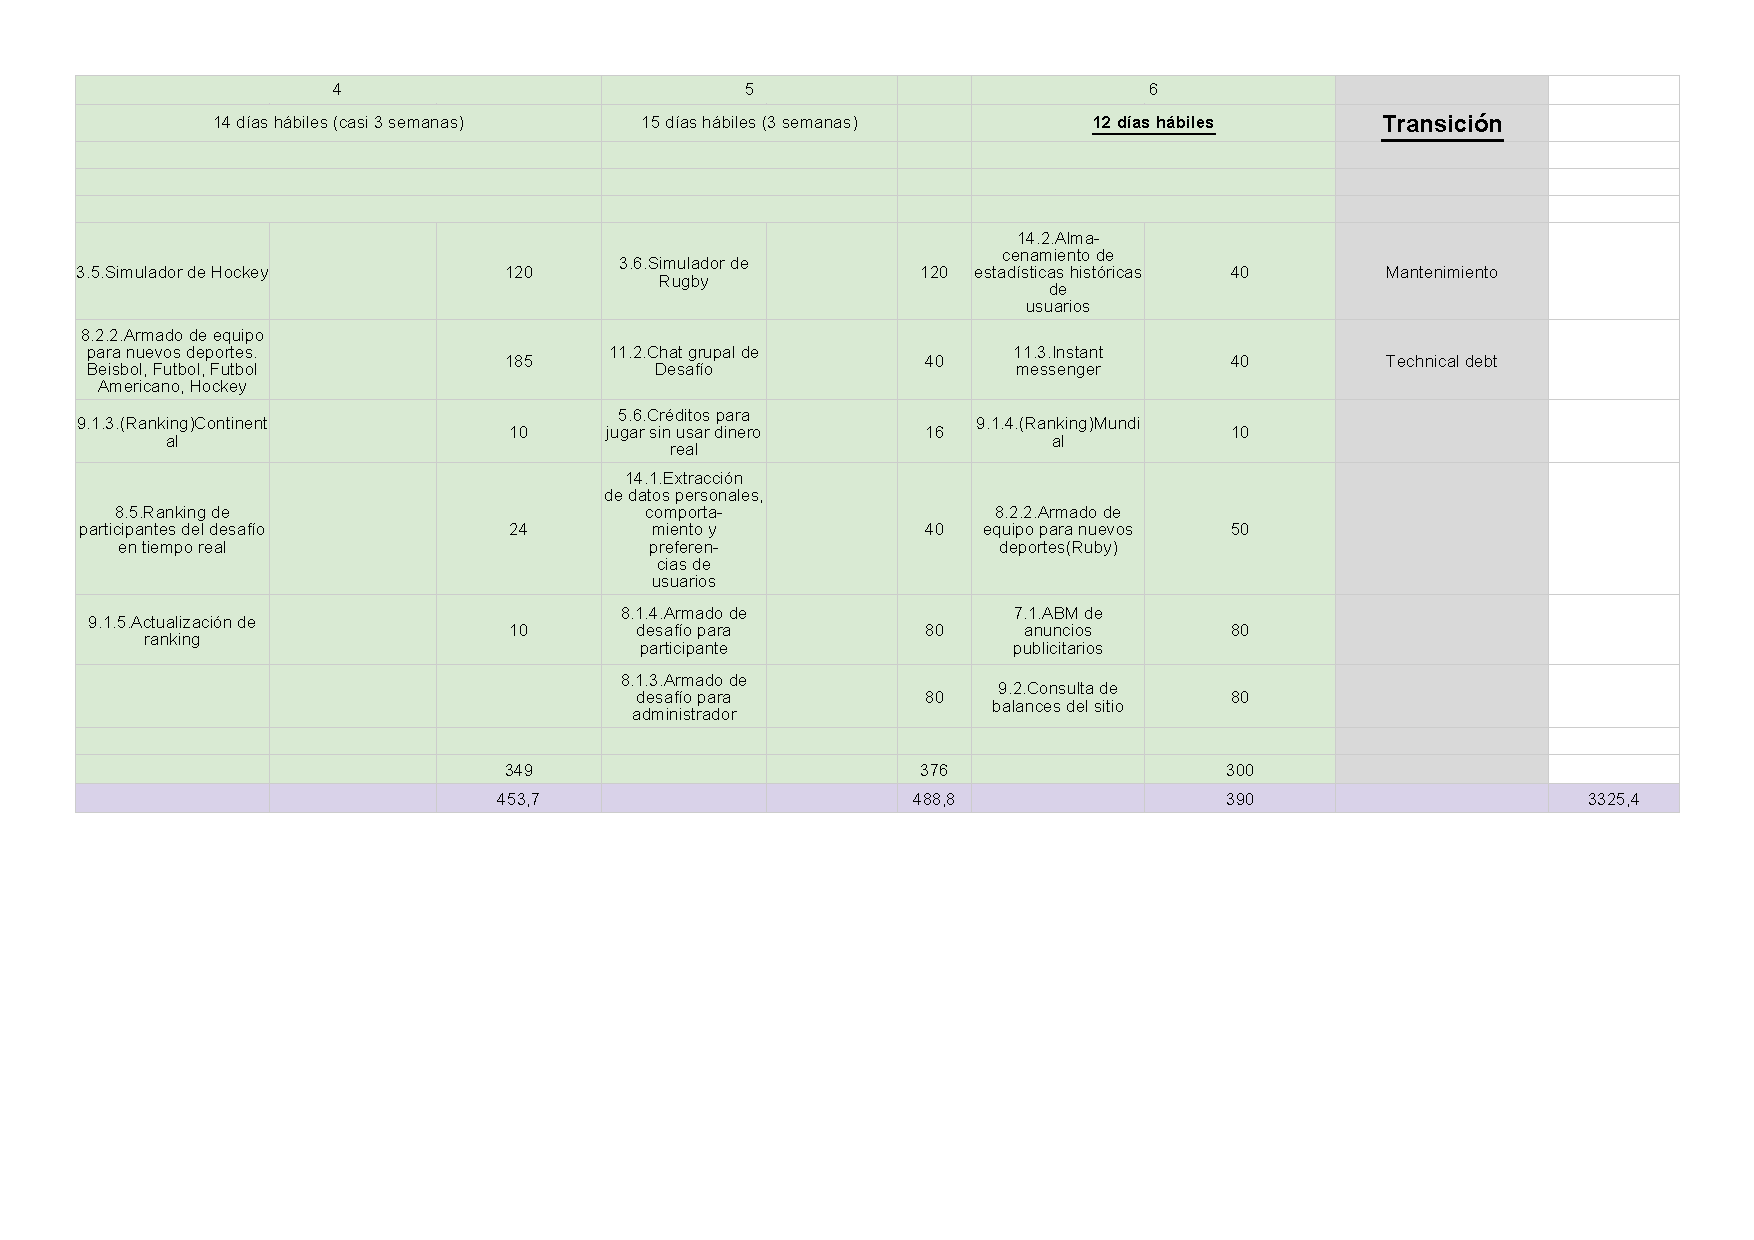
\includegraphics[scale=0.8]{imagenes/construccion-transicion.pdf}
   \caption{División de tareas de las últimas 3 iteraciones de la etapa de 'Construcción' y 'Transicion'}
\end{figure}

\end{landscape}
\newpage



